\section{現状の課題}

近年、日本国内ではeスポーツの市場規模やファン人口が増加しており、大会や地域イベントも開催されるようになっています。
一般社団法人日本eスポーツ協会(JESU)によると、日本国内のeスポーツ市場規模は、2021年の78.4億円から2024年には約161億円に拡大し、
約2.1倍となっています。また、2024年の市場ではイベント運営が37.3\%を占めています。\cite{jeSU2026} 
\footnote{[1] 一般社団法人日本eスポーツ協会，「eスポーツの市場と推移」，2026． 
 日本eスポーツ協会「eスポーツの市場と推移」（2026年10月15日閲覧）}

\begin{figure}[H]
  \centering
  \begin{tikzpicture}
    \pie[
      radius=3,
      sum=auto,
      text=pin,
      explode={0,0,0,0,0,0,0.3,0},
      color={orange!80, red!60, olive!70, lime!60!olive, violet!50, blue!40, cyan!70!blue, red!70!black}
    ]{
      9.7/{放映権},
      36.3/{スポンサー},
      1.9/{チケット},
      7.4/{アイテム課金・賞金},
      0.8/{グッズ},
      0.3/{著作権許諾},
      37.3/{イベント運営},
      6.2/{ストリーミング}
    }
  \end{tikzpicture}
  \caption{日本国内eスポーツ市場の割合（出典：一般社団法人日本eスポーツ協会，「eスポーツの市場と推移」）}
  \label{fig:revenue}
\end{figure}


さらに、国内eスポーツファン数は2021年の743万人から2024年には967万人に増加し、約30\%増加しています。
この推移を図\ref{fig:trend}に示します。

\begin{figure}[H]
  \centering
  \begin{tikzpicture}
    \begin{axis}[
      ybar,
      width=0.85\linewidth,
      height=7cm,
      bar width=1.2cm,
      symbolic x coords={2020年,2021年,2022年,2023年,2024年},
      xtick=data,
      ymin=0, ymax=10000,
      ytick={0,2000,4000,6000,8000,10000},
      scaled y ticks=false,
      yticklabel={\pgfmathprintnumber[fixed,1000 sep={,}]{\tick}},  
      title={\small （千人）},
      title style={anchor=east, at={(0,1.02)}, xshift=-0.5cm},
      nodes near coords,
      nodes near coords style={/pgf/number format/fixed, /pgf/number format/1000 sep={,}},
      ymajorgrids=true,
      grid style={dashed, gray!50},
      enlarge x limits=0.15
    ]
      \addplot[fill=violet!70!black, draw=none] coordinates {
        (2020年,6859)
        (2021年,7434)
        (2022年,7759)
        (2023年,8560)
        (2024年,9673)
      };
    \end{axis}
  \end{tikzpicture}
  \caption{日本国内eスポーツファン数の推移（出典：\cite{jeSU2026}）}
  \label{fig:trend}
\end{figure}

一方、大会運営では参加者情報や試合結果の管理が必要となります。
また、観戦者が注目選手の試合状況や次の対戦相手、大会全体の進行状況を簡単に確認できる仕組みも重要です。
そのほかにも、小規模から中規模の大会では、大会情報とライブ配信が別々に提供されるなど、
観戦者が必要な情報をまとめて確認しにくいといった問題もあります。\footnote{Esports Charts, “T1 enjoys first win in weeks and viewership boost as Faker returns from health break,” 2023年8月3日, https://escharts.com/news/t1-lcksummer2023-viewership （2026年10月15日閲覧） }

また、注目選手の参加が大会の視聴状況に影響する事例もあります。
例えば、世界中で人気を集める対戦型ゲーム「League of Legends」では、
韓国のプロチームに世界トップレベルに活躍する選手がいます。

この選手の復帰後、離脱期間中と比較してピーク視聴者数が18.4\%、平均視聴者数が19\%増加したことが報告されています\cite{escharts2023}
\footnote{[3] Esports Charts, “How League of Legends World Championship viewership has evolved over time,” Esports Charts, 2025. 
  Esports Charts （2026年10月15日閲覧） }
\begin{figure}[H]
  \centering
  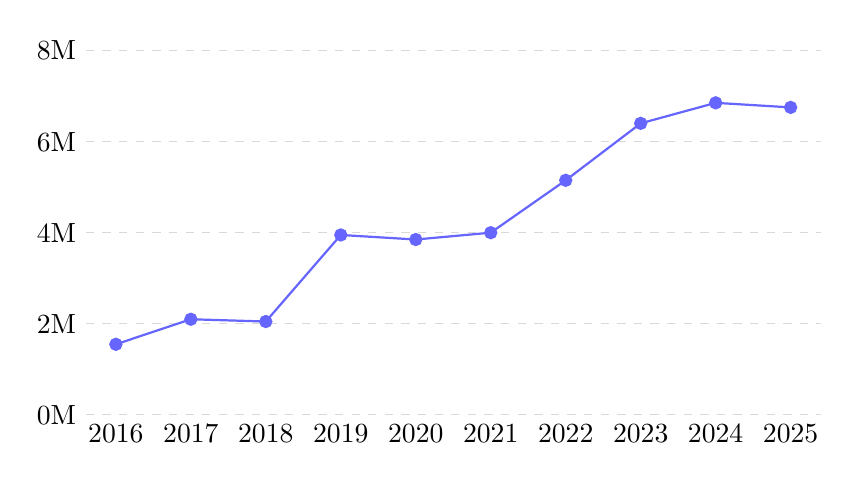
\begin{tikzpicture}
    \begin{axis}[
      width=0.9\linewidth,
      height=6.5cm,
      xmin=2015.6, xmax=2025.4,
      xtick={2016,2017,2018,2019,2020,2021,2022,2023,2024,2025},
      xticklabel style={/pgf/number format/1000 sep={}},
      ymin=0, ymax=8.5,
      ytick={0,2,4,6,8},
      scaled y ticks=false,
      yticklabel={\pgfmathprintnumber[fixed,precision=0]{\tick}M},
      ymajorgrids=true,
      grid style={dashed, gray!30},
      axis line style={draw=none},
      tick style={draw=none}
    ]
      \addplot[color=blue!60, thick, mark=*, mark options={fill=blue!60}] coordinates {
        (2016,1.55)
        (2017,2.10)
        (2018,2.05)
        (2019,3.95)
        (2020,3.85)
        (2021,4.00)
        (2022,5.15)
        (2023,6.40)
        (2024,6.85)
        (2025,6.75)
      };
    \end{axis}
  \end{tikzpicture}
  \caption{League of Legends World Championshipのピーク視聴者数の推移（単位：百万人、出典：\cite{escharts2025}）}
  \label{fig:line_trend}
\end{figure}

このことから、観戦者が注目選手の試合結果や今後の対戦予定を確認できることは、大会を継続して楽しむうえで重要であると考えられます。

一方、地域や学校、企業、ゲームコミュニティ等が主催する大会では、Discordなどのコミュニケーションツールと、
ExcelやGoogleスプレッドシートなどを組み合わせて参加者情報や試合結果を管理している例があります。
実際に、60人規模のゲーム大会で、ゲーム画面のスコアをGoogleスプレッドシートへ手入力していた事例%\cite{qiita2022}
もあり、情報の更新や共有に手作業が発生し、管理に遅れが生じることが課題となっています。
また、情報が複数のツールに分散すると、協議参加者が自分の試合情報を確認しにくくなるだけでなく、
観戦者もトーナメント表や試合結果、注目選手の対戦状況などを把握するために複数のページを確認する必要が生じます。

既存の大会運営プラットフォームには、大会作成、参加者登録、トーナメント設定、勝敗管理などの機能が提供されています。
既存のプラットフォームにおける運営の効率化だけでなく、観戦者が大会情報とライブ配信を関連付けて確認できる仕組みも重要です。
特に、小規模から中規模の大会では、専用システムの導入費用や運用費用が負担となる場合もあり、利用しやすい大会運営システムが求められています。

そこで、大会運営に必要な情報を一元管理し、主催者・競技参加者・観戦者がそれぞれ必要な情報を確認できる
「小規模ゲーム大会運営システム(Play Line)」を提案します。本システムでは、
運営者向け機能として参加登録から試合結果の管理までを効率化することを目的とし、また、運営者・観戦者向け機能として
トーナメント表、試合結果、注目選手の対戦状況、次の対戦相手およびライブ配信へのアクセスを提供します。
これにより、主催者の運営負担を軽減し、競技参加者が必要な情報を確認しやすくするとともに、観戦者が大会の進行状況や注目選手の試合を追いやすい環境の実現を目指します。